\documentclass[12pt, a4paper]{article}

%% ─── Packages ───────────────────────────────────────────────────────────────
\usepackage[utf8]{inputenc}
\usepackage[T1]{fontenc}
\usepackage[margin=2.5cm]{geometry}
\usepackage{amsmath, amssymb, amsthm}
\usepackage{mathtools}
\usepackage{graphicx}
\usepackage{tikz}
\usetikzlibrary{shapes.geometric, arrows.meta, positioning, fit, backgrounds, calc}
\usepackage{algorithm}
\usepackage{algpseudocode}
\usepackage{booktabs}
\usepackage{multirow}
\usepackage{array}
\usepackage{xcolor}
\usepackage{hyperref}
\usepackage{enumitem}
\usepackage{caption}
\usepackage{subcaption}
\usepackage{cite}
\usepackage{setspace}
\usepackage{fancyhdr}
\usepackage{titlesec}

%% ─── Colors ─────────────────────────────────────────────────────────────────
\definecolor{onapblue}{RGB}{0, 84, 166}
\definecolor{attackred}{RGB}{192, 0, 0}
\definecolor{safegreen}{RGB}{0, 128, 0}
\definecolor{warnorange}{RGB}{255, 140, 0}
\definecolor{lightgray}{RGB}{240, 240, 240}
\definecolor{darkgray}{RGB}{80, 80, 80}
\definecolor{accentpurple}{RGB}{102, 45, 145}

\hypersetup{
  colorlinks=true,
  linkcolor=onapblue,
  citecolor=onapblue,
  urlcolor=onapblue
}

%% ─── Header/Footer ──────────────────────────────────────────────────────────
\pagestyle{fancy}
\fancyhf{}
\rhead{\textcolor{darkgray}{\small AI-Augmented NFV Orchestration for Proactive DDoS Protection}}
\lhead{\textcolor{darkgray}{\small Research Proposal}}
\cfoot{\thepage}

%% ─── Title ──────────────────────────────────────────────────────────────────
\title{
  \vspace{-1cm}
  \textbf{\Large AI-Augmented NFV Orchestration for Proactive DDoS Protection\\
  in Cloud Data Centers}\\[0.5em]
  \large Research Gap, Problem Formulation, Proposed Method \& Solution Pipeline
}
\author{
  \normalsize Khóa luận tốt nghiệp --- Đề xuất Nghiên cứu
}
\date{\today}

%% ─── Document ────────────────────────────────────────────────────────────────
\begin{document}
\maketitle
\thispagestyle{fancy}
\tableofcontents
\newpage

%% ═══════════════════════════════════════════════════════════════════════════
\section{Research Gap Analysis}
%% ═══════════════════════════════════════════════════════════════════════════

\subsection{State of the Art Overview}

Distributed Denial-of-Service (DDoS) attack defense has evolved significantly
over the past decade. Existing approaches can be classified along two orthogonal
axes: (i)~\textit{the AI/ML technique employed}, and (ii)~\textit{the network
management layer targeted}.

\begin{table}[h!]
\centering
\caption{Comparative analysis of related work (representative papers, 2018--2025).}
\label{tab:related_work}
\setlength{\tabcolsep}{4pt}
\renewcommand{\arraystretch}{1.25}
\begin{tabular}{@{}p{4.5cm} c c c c c c@{}}
\toprule
\textbf{Work} & \textbf{AI/ML} & \textbf{NFV} & \textbf{MANO} & \textbf{Proactive} &
\textbf{Cloud DC} & \textbf{Closed Loop} \\
\midrule
Zhou et al.~(2017)          & \texttimes & \checkmark & \texttimes & \texttimes & \texttimes & \texttimes \\
DeMONS~(2018)               & \texttimes & \checkmark & \texttimes & \texttimes & \texttimes & \texttimes \\
LUCID~(2020)                & CNN        & \texttimes & \texttimes & \texttimes & \texttimes & \texttimes \\
ORACLE~(2020)               & KNN        & \texttimes & \texttimes & \texttimes & \texttimes & \texttimes \\
Sultana et al.~(2021)       & ML         & \checkmark & ONAP       & \texttimes & \texttimes & Partial    \\
z-TORCH~(2018)              & ML         & \checkmark & MANO       & \texttimes & \checkmark & \checkmark \\
Yungaicela et al.~(2023)    & RL         & \checkmark & \texttimes & \texttimes & \texttimes & \texttimes \\
TSP\_CSSE~(2024)            & RF/XGB     & \checkmark & K8s        & \texttimes & \checkmark & \texttimes \\
De Oliveira et al.~(2023)   & ML         & \checkmark & \texttimes & \texttimes & \texttimes & \texttimes \\
Zein et al.~(2025)          & XAI/DL     & \checkmark & MANO       & \texttimes & \texttimes & Reactive   \\
Chen \& Hsieh~(2025)        & ML         & \checkmark & ONAP       & \texttimes & \checkmark & Partial    \\
Cross-layer~(2025)          & DL         & \checkmark & NFVO       & Partial    & \texttimes & \texttimes \\
\midrule
\textbf{This work}          & \textbf{LSTM+RF} & \checkmark & \textbf{ONAP} &
\checkmark & \checkmark & \checkmark \\
\bottomrule
\end{tabular}
\end{table}

\subsection{Identified Research Gaps}

Based on the systematic review of 29 papers (Table~\ref{tab:related_work}),
the following critical research gaps are identified:

\begin{description}[leftmargin=1.5cm, labelwidth=1.2cm, font=\bfseries\color{attackred}]

\item[Gap 1.] \textbf{No proactive DDoS defense on a production-grade MANO
platform.}
The vast majority of works either propose reactive defenses (detection
precedes mitigation) or test on simulation environments (Mininet,
Containernet). No work integrates a \textit{time-series prediction} model
directly into the \textit{ONAP DCAE} analytics pipeline to trigger
pre-provisioning of security VNFs before attack traffic saturates
infrastructure resources.

\item[Gap 2.] \textbf{No attack-type-aware VNF chain selection in MANO.}
Existing NFV-based mitigation systems deploy a single, generic mitigation
VNF regardless of attack type. The relationship between the specific DDoS
attack category (volumetric, protocol-exploit, slow-rate, application-layer)
and the optimal security VNF chain composition has not been explored in the
MANO orchestration context.

\item[Gap 3.] \textbf{Absence of a closed-loop retraining feedback mechanism
in ONAP for DDoS defense.}
While z-TORCH~\cite{zTORCH2018} demonstrated closed-loop feedback for VNF
placement optimization, no work applies this principle specifically for
continuous improvement of DDoS detection and prediction models deployed
within ONAP. Models become stale as attack patterns evolve (concept drift).

\item[Gap 4.] \textbf{Cloud data center context is underserved.}
Works focusing on MEC~\cite{guo2021nfv} or 5G networks~\cite{zein2025reactive}
do not address the unique characteristics of cloud data centers:
multi-tenancy, east-west traffic dominance, shared resource pools, and
ONAP-managed VNF lifecycle.

\end{description}

%% ═══════════════════════════════════════════════════════════════════════════
\section{Research Questions}
%% ═══════════════════════════════════════════════════════════════════════════

Addressing the four gaps above, this thesis poses the following research questions:

\begin{description}[leftmargin=1.5cm, labelwidth=1.2cm,
                    font=\normalfont\bfseries\color{onapblue}]

\item[RQ1.] \textit{(Proactive Prediction)} Can a time-series model (LSTM/TCN)
deployed as an ONAP DCAE microservice accurately predict DDoS attack
probability 30--60 seconds in advance, providing a sufficient pre-provisioning
window for security VNFs?

\item[RQ2.] \textit{(Attack Classification)} Can an efficient ML classifier
(Random Forest / XGBoost) identify the DDoS attack category from early-stage
traffic features with accuracy $\geq$\,97\% and inference latency
$<$\,10\,ms, enabling timely selection of the appropriate VNF chain template?

\item[RQ3.] \textit{(Orchestration Automation)} Can an ONAP CLAMP policy,
driven by the outputs of RQ1 and RQ2, automatically instantiate the correct
security VNF chain via ONAP SO with a provisioning time that reduces
legitimate-traffic disruption by at least 50\% compared to reactive baselines?

\item[RQ4.] \textit{(Adaptive Closed Loop)} Does a closed-loop feedback
mechanism that retrains the predictor and classifier from post-mitigation
labeled traffic improve detection performance over time, demonstrating
resilience to concept drift?

\end{description}

%% ═══════════════════════════════════════════════════════════════════════════
\section{Problem Formulation}
%% ═══════════════════════════════════════════════════════════════════════════

\subsection{System Model}

Consider a cloud data center managed by an ONAP MANO stack. The infrastructure
comprises a set of physical hosts $\mathcal{H} = \{h_1, h_2, \ldots, h_N\}$,
a pool of deployable VNF instances $\mathcal{V} = \{v_1, v_2, \ldots, v_M\}$,
and an SDN-controlled network fabric. Network traffic is observed via
distributed probes (sFlow/IPFIX) that export per-flow statistics to DCAE.

Let $\mathbf{x}_t \in \mathbb{R}^F$ denote the traffic feature vector at
discrete time step $t$, where $F$ is the number of extracted features
(e.g., packet rate, byte rate, SYN count, source-IP entropy, flow count).
The observation window of length $W$ is:
\begin{equation}
  \mathbf{X}_{t-W:t} = \bigl[\mathbf{x}_{t-W},\; \mathbf{x}_{t-W+1},\; \ldots,\; \mathbf{x}_{t}\bigr]
  \in \mathbb{R}^{W \times F}.
  \label{eq:obs_window}
\end{equation}

\subsection{Prediction Sub-problem}

\textbf{Definition 1 (Attack Probability Forecast).}
Given the observation window $\mathbf{X}_{t-W:t}$, the predictor $f_\theta$
produces a probability score for the future horizon $\Delta$ time steps ahead:
\begin{equation}
  \hat{p}_{t+\Delta} = f_\theta\!\left(\mathbf{X}_{t-W:t}\right) \in [0, 1],
  \label{eq:predictor}
\end{equation}
where $\theta$ are learnable parameters of the LSTM/TCN model and $\Delta$
is the \textit{pre-provisioning lead time} (target: $\Delta \in [30, 60]$
seconds). The system raises a \textit{pre-alert} when
$\hat{p}_{t+\Delta} > \tau_{\mathrm{pre}}$.

\subsection{Classification Sub-problem}

\textbf{Definition 2 (Attack-Type Classification).}
Upon pre-alert, the classifier $g_\phi$ maps the current feature vector to
one of $K$ attack categories:
\begin{equation}
  \hat{k}_t = \arg\max_{k \in \mathcal{K}}\; g_\phi\!\left(\mathbf{x}_t\right),
  \label{eq:classifier}
\end{equation}
where $\mathcal{K} = \{\text{Volumetric},\, \text{Protocol},\,
\text{Slow-Rate},\, \text{Application}\}$ and $\phi$ are the classifier
parameters.

\subsection{VNF Chain Selection}

\textbf{Definition 3 (VNF Chain Template).}
A VNF chain template $\mathcal{C}_k$ is an ordered sequence of VNF types
selected for attack category $k$:
\begin{equation}
  \mathcal{C}\!: \mathcal{K} \rightarrow 2^{\mathcal{V}},
  \qquad
  \mathcal{C}_k = \bigl(v^{(1)}_k,\; v^{(2)}_k,\; \ldots,\; v^{(n_k)}_k\bigr),
  \label{eq:vnf_template}
\end{equation}
where traffic traverses the chain in order. The four templates are:
\begin{align}
  \mathcal{C}_{\text{Vol}}   &= (\text{RateLimiter},\; \text{Scrubber}) \label{eq:tmpl1}\\
  \mathcal{C}_{\text{Proto}} &= (\text{StatefulFW},\; \text{IDS}) \label{eq:tmpl2}\\
  \mathcal{C}_{\text{Slow}}  &= (\text{DPI},\; \text{BehaviorAnalyzer}) \label{eq:tmpl3}\\
  \mathcal{C}_{\text{App}}   &= (\text{WAF},\; \text{RateLimiter}) \label{eq:tmpl4}
\end{align}

\subsection{Optimization Objective}

The overall system objective balances protection effectiveness against
resource cost and false-alarm penalty:

\begin{equation}
  \underset{\theta,\,\phi,\,\boldsymbol{\tau}}{\text{minimize}}\quad
  \underbrace{\alpha \cdot D_{\mathrm{svc}}}_{\text{disruption}} \;+\;
  \underbrace{\beta \cdot R_{\mathrm{ovp}}}_{\text{over-provision}} \;+\;
  \underbrace{\gamma \cdot \mathcal{L}_{\mathrm{FA}}}_{\text{false alarm}},
  \label{eq:objective}
\end{equation}

\noindent subject to:
\begin{align}
  \text{(C1)}\quad & T_{\mathrm{prov}} < \Delta \cdot s_{\mathrm{step}}
    \quad \text{(VNF ready before attack peak)}, \label{eq:c1}\\
  \text{(C2)}\quad & \text{F1}_{\hat{k}} \geq 0.97
    \quad \text{(classifier accuracy)}, \label{eq:c2}\\
  \text{(C3)}\quad & \text{FPR}_{\hat{p}} \leq 0.05
    \quad \text{(predictor false positive rate)}, \label{eq:c3}\\
  \text{(C4)}\quad & \sum_{v \in \mathcal{C}_{\hat{k}}} r_v \leq R_{\mathrm{avail}}
    \quad \text{(resource feasibility)},\label{eq:c4}
\end{align}

\noindent where $D_{\mathrm{svc}}$ is service disruption time,
$R_{\mathrm{ovp}}$ is the fraction of wasted provisioned resources,
$\mathcal{L}_{\mathrm{FA}}$ is the false-alarm count, $T_{\mathrm{prov}}$
is VNF chain instantiation latency, $s_{\mathrm{step}}$ is the monitoring
interval, and $r_v$ is the resource demand of VNF $v$.

%% ═══════════════════════════════════════════════════════════════════════════
\section{Proposed Method}
%% ═══════════════════════════════════════════════════════════════════════════

\subsection{System Architecture}

The proposed system, named \textbf{PAD-ONAP}
(\underline{P}roactive \underline{A}I-driven \underline{D}DoS Defense
on \underline{ONAP}), maps directly onto the standard ONAP component stack
and extends it with three new AI microservices in DCAE, one CLAMP policy
blueprint, and a feedback retraining service.

\begin{figure}[h!]
\centering
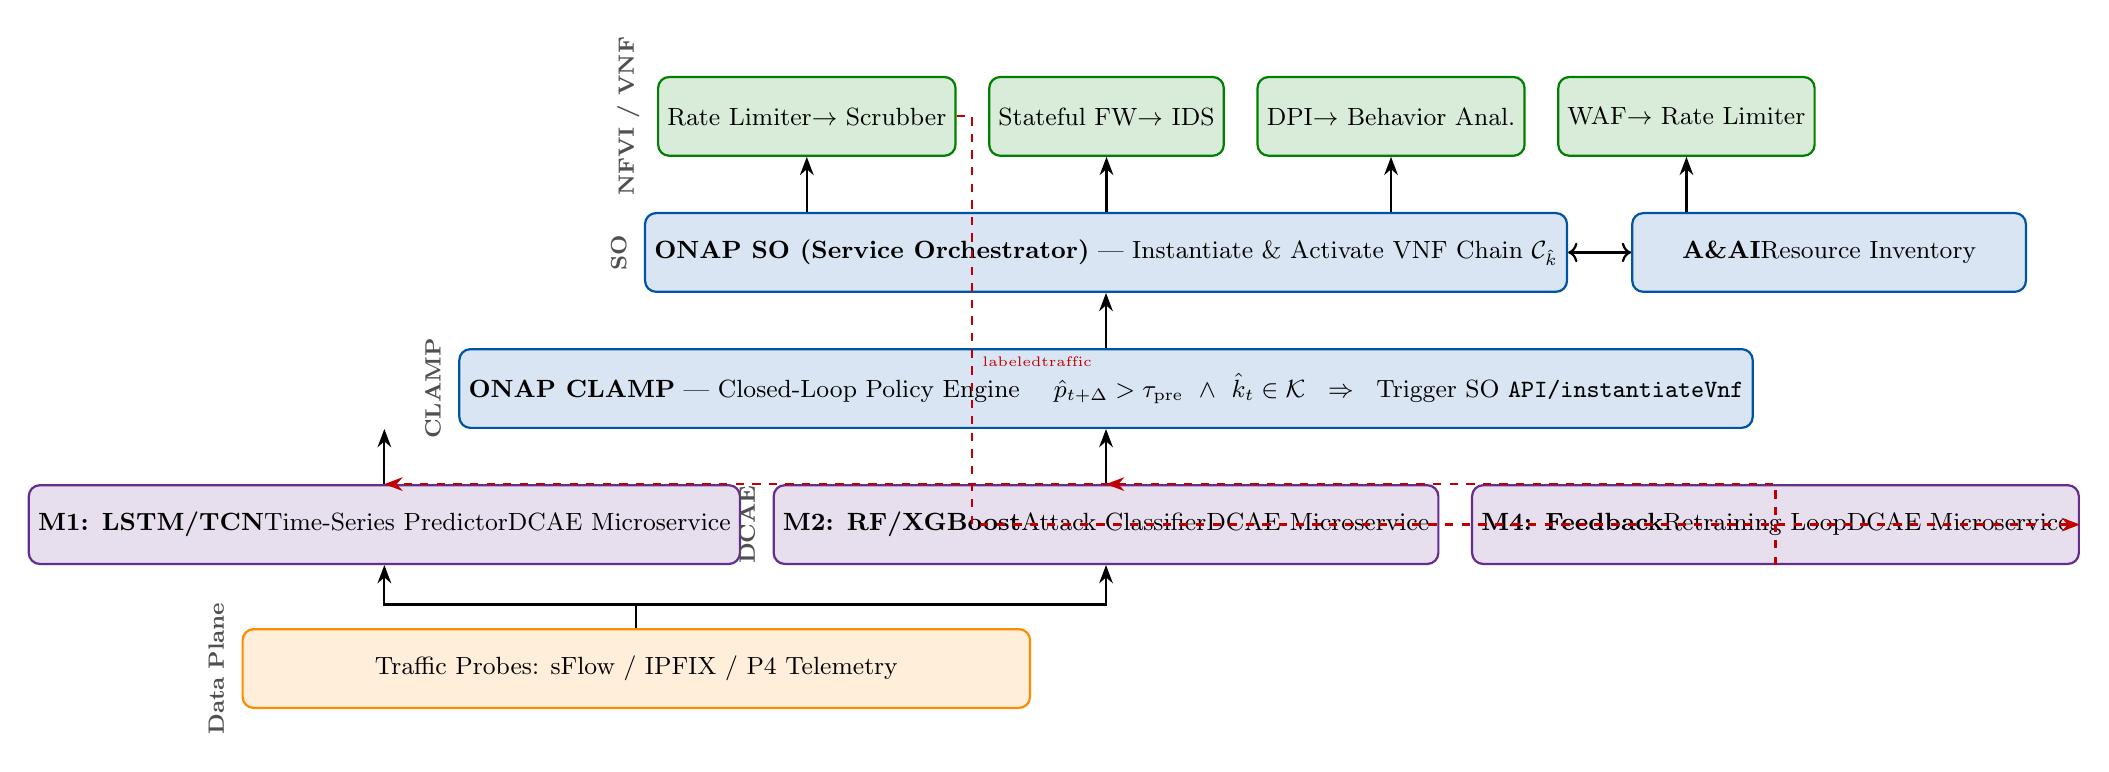
\begin{tikzpicture}[
  node distance = 0.6cm and 1.2cm,
  box/.style     = {rectangle, rounded corners=4pt, draw, thick,
                    minimum height=1.0cm, text centered, font=\small},
  onapbox/.style = {box, fill=onapblue!15, draw=onapblue},
  aibox/.style   = {box, fill=accentpurple!15, draw=accentpurple},
  vnfbox/.style  = {box, fill=safegreen!15, draw=safegreen},
  databox/.style = {box, fill=warnorange!15, draw=warnorange},
  arrow/.style   = {-Stealth, thick},
  dasharrow/.style = {-Stealth, thick, dashed}
]

%% Data plane
\node[databox, minimum width=10cm] (probes)
  {Traffic Probes: sFlow / IPFIX / P4 Telemetry};

%% DCAE layer
\node[aibox, minimum width=3.2cm, above=0.8cm of probes, xshift=-3.2cm] (predictor)
  {\textbf{M1: LSTM/TCN}\\\small Time-Series Predictor\\\small DCAE Microservice};

\node[aibox, minimum width=3.2cm, right=0.4cm of predictor] (classifier)
  {\textbf{M2: RF/XGBoost}\\\small Attack Classifier\\\small DCAE Microservice};

\node[aibox, minimum width=3.2cm, right=0.4cm of classifier] (retrain)
  {\textbf{M4: Feedback}\\\small Retraining Loop\\\small DCAE Microservice};

%% CLAMP
\node[onapbox, minimum width=10cm, above=0.7cm of classifier] (clamp)
  {\textbf{ONAP CLAMP} --- Closed-Loop Policy Engine
   \quad $\hat{p}_{t+\Delta} > \tau_{\mathrm{pre}}$ \;$\wedge$\;
   $\hat{k}_t \in \mathcal{K}$ \;\;$\Rightarrow$\;\;
   Trigger SO \texttt{API/instantiateVnf}};

%% SO
\node[onapbox, minimum width=10cm, above=0.7cm of clamp] (so)
  {\textbf{ONAP SO (Service Orchestrator)} ---
   Instantiate \& Activate VNF Chain $\mathcal{C}_{\hat{k}}$};

%% VNF chains row
\node[vnfbox, minimum width=2.0cm, above=0.7cm of so, xshift=-3.8cm] (vol)
  {\small Rate Limiter\\$\rightarrow$ Scrubber};
\node[vnfbox, minimum width=2.0cm, right=0.4cm of vol] (proto)
  {\small Stateful FW\\$\rightarrow$ IDS};
\node[vnfbox, minimum width=2.0cm, right=0.4cm of proto] (slow)
  {\small DPI\\$\rightarrow$ Behavior Anal.};
\node[vnfbox, minimum width=2.0cm, right=0.4cm of slow] (app)
  {\small WAF\\$\rightarrow$ Rate Limiter};

%% A&AI
\node[onapbox, minimum width=5.0cm, right=0.8cm of so] (aai)
  {\textbf{A\&AI}\\Resource Inventory};

%% Arrows
\draw[arrow] (probes.north) -- ++(0,0.3) -| (predictor.south);
\draw[arrow] (probes.north) -- ++(0,0.3) -| (classifier.south);
\draw[arrow] (predictor.north) -- (clamp.south -| predictor);
\draw[arrow] (classifier.north) -- (clamp.south -| classifier);
\draw[arrow] (clamp.north) -- (so.south);
\draw[arrow] (so.north -| vol.south) -- (vol.south);
\draw[arrow] (so.north -| proto.south) -- (proto.south);
\draw[arrow] (so.north -| slow.south) -- (slow.south);
\draw[arrow] (so.north -| app.south) -- (app.south);
\draw[arrow, <->] (so.east) -- (aai.west);

%% Feedback dashed
\draw[dasharrow, color=attackred] (vol.east) -- ++(0.2,0)
  |- node[pos=0.3, right, font=\tiny, color=attackred]
  {labeled\\ traffic} (retrain.east);
\draw[dasharrow, color=attackred] (retrain.south) -- (classifier.north -| retrain)
  -- (classifier.north);
\draw[dasharrow, color=attackred] (retrain.south) -- (predictor.north -| retrain)
  -- (predictor.north);

%% Labels
\node[font=\footnotesize\bfseries, color=darkgray, left=0.1cm of probes]
  {\rotatebox{90}{Data\;Plane}};
\node[font=\footnotesize\bfseries, color=darkgray, left=0.1cm of classifier]
  {\rotatebox{90}{DCAE}};
\node[font=\footnotesize\bfseries, color=darkgray, left=0.1cm of clamp]
  {\rotatebox{90}{CLAMP}};
\node[font=\footnotesize\bfseries, color=darkgray, left=0.1cm of so]
  {\rotatebox{90}{SO}};
\node[font=\footnotesize\bfseries, color=darkgray, left=0.1cm of vol]
  {\rotatebox{90}{NFVI / VNF}};

\end{tikzpicture}
\caption{PAD-ONAP Architecture: four modules mapped onto ONAP components.
         Red dashed arrows denote the feedback/retraining closed loop.}
\label{fig:architecture}
\end{figure}

\subsection{Module 1: LSTM/TCN Time-Series Predictor (M1)}

\subsubsection{Model Architecture}

The predictor is a Temporal Convolutional Network (TCN) with residual
connections, chosen over vanilla LSTM for its parallelizable training and
superior long-range dependency capture. The input is the sliding window
$\mathbf{X}_{t-W:t}$ from Eq.~\eqref{eq:obs_window} with $W = 30$ steps
($= 90$\,seconds at 3\,s polling interval).

\begin{equation}
  \hat{p}_{t+\Delta} = \sigma\!\left(
    \mathbf{w}^\top \cdot \mathrm{TCN}\!\left(\mathbf{X}_{t-W:t};\,\boldsymbol\Theta\right)
    + b
  \right),
  \label{eq:tcn}
\end{equation}

\noindent where $\sigma(\cdot)$ is the sigmoid function, $\mathbf{w}$ and $b$
are output-layer parameters, and $\boldsymbol\Theta$ are the TCN parameters
optimized by minimizing binary cross-entropy with focal weighting to handle
class imbalance:
\begin{equation}
  \mathcal{L}_{\mathrm{focal}}(\hat{p}, y) =
  -\alpha_t (1 - \hat{p}_t)^\gamma y \log\hat{p}
  - (1 - y)\log(1 - \hat{p}),
  \label{eq:focal}
\end{equation}
with $\gamma = 2$ (focusing parameter) and $\alpha_t$ adjusted for imbalance.

\subsubsection{Two-Stage Alert Mechanism}
\begin{align}
  \text{Pre-alert (warm standby):} &\quad \hat{p}_{t+\Delta} > \tau_{\mathrm{pre}} = 0.60 \label{eq:pre}\\
  \text{Full alert (chain activate):} &\quad \hat{p}_{t+\Delta} > \tau_{\mathrm{full}} = 0.80 \label{eq:full}
\end{align}
At pre-alert, ONAP SO instantiates VNFs in warm-standby mode (resources
reserved, traffic not yet redirected). At full alert, traffic is steered
through the active chain. This two-stage approach minimizes Resource
over-provisioning from false alarms.

\subsection{Module 2: Attack Classifier (M2)}

\subsubsection{Feature Engineering}

Fifteen features are selected via Ensemble Feature Selection (majority voting
across Information Gain, SHAP importance, and Mutual Information filters,
following \cite{saha2022}):

\[
\mathbf{x}_t = \bigl[
  r_{\mathrm{pkt}},\; r_{\mathrm{byte}},\; r_{\mathrm{SYN}},\;
  H_{\mathrm{src}},\; H_{\mathrm{dst}},\; \mu_L,\; \sigma_L,\;
  r_{\mathrm{flow}},\; \mathrm{IAT}_{\mu},\; \mathrm{IAT}_{\sigma},\;
  \mathrm{TCP}_{\mathrm{flag}},\; r_{\mathrm{retry}},\;
  r_{\mathrm{ICMP}},\; r_{\mathrm{UDP}},\; r_{\mathrm{HTTP}}
\bigr]
\]

\noindent where $H$ denotes Shannon entropy, $r$ are rate metrics,
and $\mathrm{IAT}$ is inter-arrival time.

\subsubsection{Ensemble Classifier}

A soft-voting ensemble of XGBoost and Random Forest is used:
\begin{equation}
  \hat{k}_t = \arg\max_{k}\;\left[
    \lambda\, P_{\mathrm{XGB}}(k \mid \mathbf{x}_t) +
    (1-\lambda)\, P_{\mathrm{RF}}(k \mid \mathbf{x}_t)
  \right],
  \label{eq:ensemble}
\end{equation}
with $\lambda = 0.5$ (tuned via cross-validation). Target: F1\,$\geq\,0.97$,
inference latency\,$<\,10$\,ms.

\subsection{Module 3: CLAMP Policy Engine (M3)}

CLAMP (Closed-Loop Automation Management Platform) defines a TOSCA-based
policy blueprint parameterized by the outputs of M1 and M2:

\begin{algorithm}[H]
\caption{PAD-ONAP CLAMP Policy Execution}
\label{alg:clamp}
\begin{algorithmic}[1]
\Require $\hat{p}_{t+\Delta}$, $\hat{k}_t$, thresholds $\tau_{\mathrm{pre}}$,
         $\tau_{\mathrm{full}}$, chain map $\mathcal{C}$
\Ensure  Appropriate VNF chain instantiated or deactivated

\State Receive event from DCAE Message Router (Kafka topic \texttt{pad.events})
\If{$\hat{p}_{t+\Delta} > \tau_{\mathrm{full}}$}
  \State $\mathcal{C}_{\mathrm{sel}} \gets \mathcal{C}[\hat{k}_t]$ \Comment{Attack-type VNF chain}
  \State \Call{SoActivateChain}{$\mathcal{C}_{\mathrm{sel}}$, mode=\textsc{Active}}
  \State Log event to A\&AI and AAF audit trail
\ElsIf{$\hat{p}_{t+\Delta} > \tau_{\mathrm{pre}}$}
  \State $\mathcal{C}_{\mathrm{sel}} \gets \mathcal{C}[\hat{k}_t]$
  \State \Call{SoActivateChain}{$\mathcal{C}_{\mathrm{sel}}$, mode=\textsc{Standby}}
  \Comment{Reserve resources, no traffic redirect}
\Else
  \If{existing chain is active}
    \State \Call{SoTerminateChain}{$\mathcal{C}_{\mathrm{sel}}$}
    \Comment{Scale-down after attack subsides}
  \EndIf
\EndIf
\end{algorithmic}
\end{algorithm}

\subsection{Module 4: Feedback \& Retraining Loop (M4)}

After each attack event, labeled traffic samples are collected and used to
periodically retrain both M1 and M2. Let $\mathcal{D}_{\mathrm{new}}$ be
the newly labeled dataset from the post-mitigation window. The updated model
parameters are obtained via incremental learning:

\begin{equation}
  \theta^{(i+1)} = \theta^{(i)} - \eta\,
  \nabla_\theta\,\mathcal{L}\!\left(f_{\theta^{(i)}},\, \mathcal{D}_{\mathrm{new}}\right),
  \label{eq:retrain}
\end{equation}
with early stopping on a held-out validation set to prevent overfitting on
recent attack samples and catastrophic forgetting of historical patterns.
Retraining is triggered by: (a)~a completed attack event, or (b)~a weekly
scheduled update. The retrained model is deployed as a new DCAE microservice
version with A/B canary testing before full promotion.

%% ═══════════════════════════════════════════════════════════════════════════
\section{Solution Pipeline}
%% ═══════════════════════════════════════════════════════════════════════════

\subsection{End-to-End Workflow}

\begin{figure}[h!]
\centering
\begin{tikzpicture}[
  every node/.style={font=\small},
  step/.style={rectangle, rounded corners=5pt, draw=onapblue, thick,
               fill=onapblue!10, minimum width=3.0cm, minimum height=1.0cm,
               text centered, align=center},
  decision/.style={diamond, draw=warnorange, thick, fill=warnorange!10,
                   aspect=2.2, text centered, align=center, font=\footnotesize},
  action/.style={rectangle, rounded corners=5pt, draw=safegreen, thick,
                 fill=safegreen!10, minimum width=3.5cm, minimum height=0.9cm,
                 text centered, align=center},
  terminator/.style={rectangle, rounded corners=10pt, draw=darkgray, thick,
                     fill=lightgray, minimum width=2.5cm, minimum height=0.8cm,
                     text centered},
  arrow/.style={-Stealth, thick, draw=darkgray},
  node distance=0.5cm and 1.3cm
]

\node[step]   (collect) {Traffic Collection\\sFlow / IPFIX / P4};
\node[step, right=1.2cm of collect] (feat) {Feature\\Extraction (15 features)};
\node[step, right=1.2cm of feat] (pred) {M1: TCN\\Predictor\\$\hat{p}_{t+\Delta}$};
\node[decision, below=0.9cm of pred] (dec1) {$\hat{p} > \tau_{\mathrm{pre}}$?};
\node[terminator, left=1.2cm of dec1] (monitor) {Continue\\Monitoring};
\node[step, below=0.9cm of dec1] (classify) {M2: Classifier\\$\hat{k}_t$};
\node[action, below=0.9cm of classify] (standby) {SO: Pre-provision\\$\mathcal{C}_{\hat{k}}$ in Standby};
\node[decision, below=0.9cm of standby] (dec2) {$\hat{p} > \tau_{\mathrm{full}}$?};
\node[action, below=0.9cm of dec2] (activate) {SO: Activate Chain\\Redirect Traffic};
\node[step, right=1.6cm of activate] (mitigate) {VNF Chain\\Mitigates Attack};
\node[decision, right=1.6cm of mitigate] (dec3) {Attack\\Subsided?};
\node[action, above=0.9cm of dec3] (teardown) {SO: Terminate Chain\\Scale Down};
\node[step, above=0.9cm of teardown] (feedback) {M4: Label Samples\\Retrain M1 \& M2};
\node[terminator, above=0.9cm of feedback] (deploy) {Deploy Updated\\Model (DCAE)};

%% Arrows
\draw[arrow] (collect) -- (feat);
\draw[arrow] (feat) -- (pred);
\draw[arrow] (pred) -- (dec1);
\draw[arrow] (dec1) -- node[above]{\small No} (monitor);
\draw[arrow] (dec1) -- node[right]{\small Yes} (classify);
\draw[arrow] (classify) -- (standby);
\draw[arrow] (standby) -- (dec2);
\draw[arrow] (dec2.west) -- ++(-0.8,0) |- node[pos=0.25, left, font=\tiny]{Wait} (pred.west);
\draw[arrow] (dec2) -- node[right]{\small Yes}(activate);
\draw[arrow] (activate) -- (mitigate);
\draw[arrow] (mitigate) -- (dec3);
\draw[arrow] (dec3) -- node[right]{\small Yes} (teardown);
\draw[arrow] (dec3.east) -- ++(0.5,0) |- node[pos=0.1, right, font=\tiny]{No} (mitigate.east);
\draw[arrow] (teardown) -- (feedback);
\draw[arrow] (feedback) -- (deploy);
\draw[arrow] (monitor.south) -- ++(0,-0.3) -| (collect.south);
\draw[arrow] (deploy.west) -- ++(-8.5,0) |- (collect.north);

\end{tikzpicture}
\caption{PAD-ONAP end-to-end solution pipeline.}
\label{fig:pipeline}
\end{figure}

\subsection{Data Flow Specification}

Table~\ref{tab:dataflow} summarizes the inter-component data flows,
corresponding ONAP APIs, and timing requirements.

\begin{table}[h!]
\centering
\caption{Inter-component data flows and API mappings.}
\label{tab:dataflow}
\renewcommand{\arraystretch}{1.3}
\begin{tabular}{@{}lllcc@{}}
\toprule
\textbf{From} & \textbf{To} & \textbf{ONAP Interface / Protocol} & \textbf{Dir.} & \textbf{Latency Target} \\
\midrule
Data Plane Probes & DCAE (M1, M2) & \texttt{VES} over HTTPS & $\rightarrow$ & $<$\,1\,s \\
M1 Predictor      & CLAMP        & Kafka / DMaaP topic      & $\rightarrow$ & $<$\,100\,ms \\
M2 Classifier     & CLAMP        & Kafka / DMaaP topic      & $\rightarrow$ & $<$\,10\,ms \\
CLAMP Policy      & ONAP SO      & REST \texttt{/instantiateVnf} & $\rightarrow$ & $<$\,200\,ms \\
ONAP SO           & A\&AI        & REST CRUD                & $\leftrightarrow$ & $<$\,100\,ms \\
ONAP SO           & SDN-C        & NETCONF/RESTCONF         & $\rightarrow$ & $<$\,500\,ms \\
VNF Instances     & M4 Retrainer & Object Storage (S3-like) & $\rightarrow$ & async \\
M4 Retrainer      & DCAE (M1,M2) & Model Registry REST      & $\rightarrow$ & async \\
\bottomrule
\end{tabular}
\end{table}

\subsection{VNF Chain Templates Specification}

\begin{table}[h!]
\centering
\caption{Attack-type to VNF chain mapping ($\mathcal{C}: \mathcal{K} \to 2^{\mathcal{V}}$).}
\label{tab:vnf_chains}
\renewcommand{\arraystretch}{1.35}
\begin{tabular}{@{}lp{4.5cm}p{4.5cm}c@{}}
\toprule
\textbf{Attack Type} & \textbf{VNF Chain} & \textbf{Mitigation Logic} & \textbf{Avg. Prov. Time} \\
\midrule
Volumetric ($\mathcal{C}_{\text{Vol}}$)
  & Rate Limiter $\to$ Scrubber VNF
  & Drop traffic exceeding token-bucket rate; clean and forward legitimate flows
  & $\sim$8\,s \\
\addlinespace
Protocol ($\mathcal{C}_{\text{Proto}}$)
  & Stateful FW $\to$ IDS VNF
  & Block malformed packets; deep-inspect protocol compliance; reset bad sessions
  & $\sim$10\,s \\
\addlinespace
Slow-Rate ($\mathcal{C}_{\text{Slow}}$)
  & DPI VNF $\to$ Behavior Analyzer
  & Detect slow-connection exhaustion patterns; score and blacklist slow-sender IPs
  & $\sim$12\,s \\
\addlinespace
Application ($\mathcal{C}_{\text{App}}$)
  & WAF $\to$ Rate Limiter VNF
  & Filter malicious HTTP/HTTPS requests; rate-limit per-URI endpoints
  & $\sim$9\,s \\
\bottomrule
\end{tabular}
\end{table}

\subsection{Experimental Design}

\subsubsection{Testbed}
The system is deployed on the existing \textbf{ONAP + NFV infrastructure}
with the following configuration:
\begin{itemize}[noitemsep]
  \item ONAP components: DCAE, CLAMP, SO, A\&AI, SDN-C, Policy Framework
  \item NFV Compute: OpenStack-managed VMs for VNF hosting
  \item Networking: OpenDaylight SDN controller, OpenFlow 1.3
  \item Traffic Generation: D-ITG, Scapy-based DDoS emulator,
        replayed CICDDoS2019 traces
\end{itemize}

\subsubsection{Datasets}
\begin{itemize}[noitemsep]
  \item \textbf{CICDDoS2019}: 12 attack types, timestamped flows --- primary
        dataset for training/testing M1 and M2
  \item \textbf{BCCC-cPacket-Cloud-DDoS-2024}: cloud-specific DDoS traces ---
        used for cloud scenario generalization testing
  \item \textbf{Custom synthetic traces}: generated by replaying above
        datasets via D-ITG at variable rates to simulate real-time arrival
\end{itemize}

\subsubsection{Evaluation Metrics}
\begin{equation}
\text{Metrics} =
\begin{cases}
  \Delta_{\mathrm{lead}} = T_{\mathrm{attack\_peak}} - T_{\mathrm{vnf\_ready}}
    & \text{(pre-emptive lead time, target $> 0$\,s)} \\[4pt]
  D_{\mathrm{svc}} = \int_{t_{\mathrm{atk}}}^{t_{\mathrm{mit}}}
    \!\!\bigl(1 - \rho_{\mathrm{legit}}(t)\bigr)\,dt
    & \text{(service disruption, seconds)} \\[4pt]
  \text{F1}_{\hat{k}} = \frac{2\,\mathrm{TP}}{2\,\mathrm{TP} + \mathrm{FP} + \mathrm{FN}}
    & \text{(per-class attack detection F1)} \\[4pt]
  \mathrm{FPR} = \frac{\mathrm{FP}}{\mathrm{FP} + \mathrm{TN}}
    & \text{(false alarm rate, target $\leq 5\%$)} \\[4pt]
  R_{\mathrm{eff}} = 1 - \frac{R_{\mathrm{wasted}}}{R_{\mathrm{provisioned}}}
    & \text{(resource utilization efficiency)}
\end{cases}
\label{eq:metrics}
\end{equation}

\subsubsection{Baselines for Comparison}
\begin{enumerate}[noitemsep, label=\textbf{B\arabic*.}]
  \item \textbf{Reactive-ONAP}: same ONAP stack but detection triggers VNF
        instantiation (no prediction) --- measures raw provisioning delay gap
  \item \textbf{Threshold-ONAP}: simple statistical threshold on packet rate
        (no ML) triggers CLAMP --- measures ML benefit
  \item \textbf{FGCS2023} \cite{yungaicela2023}: RL+MTD framework from
        Yungaicela-Naula et al.\ --- measures RL vs.\ predictive approach
  \item \textbf{PAD-ONAP (no feedback)}: ablation --- M4 disabled to
        quantify the benefit of the retraining loop
\end{enumerate}

%% ═══════════════════════════════════════════════════════════════════════════
\section{Expected Contributions}
%% ═══════════════════════════════════════════════════════════════════════════

This thesis makes the following \textbf{four original contributions}:

\begin{enumerate}[label=\textbf{C\arabic*.}, leftmargin=1.5cm]

\item \textbf{First proactive DDoS defense system fully integrated into ONAP
MANO for cloud data centers.} Unlike prior work that either uses ONAP for
generic anomaly detection or proposes proactive defense in simulation-only
environments, PAD-ONAP delivers end-to-end proactivity on a production-grade
orchestration platform.

\item \textbf{A novel attack-type-aware VNF chain selection mechanism.}
The mapping $\mathcal{C}: \mathcal{K} \to 2^{\mathcal{V}}$
(Eq.~\eqref{eq:vnf_template}) enables targeted, efficient mitigation
by deploying only the VNFs necessary for the detected attack type,
reducing resource wastage compared to one-size-fits-all approaches.

\item \textbf{A closed-loop model retraining pipeline within ONAP DCAE.}
The Feedback Module (M4) provides adaptive resilience to concept drift,
demonstrated through longitudinal experiments measuring F1 improvement
across successive attack campaigns.

\item \textbf{Quantitative characterization of the pre-provisioning benefit.}
Using the metric $\Delta_{\mathrm{lead}}$ and $D_{\mathrm{svc}}$, this work
provides the first empirical evidence of how much proactive VNF provisioning
reduces user-visible service disruption in a cloud data center under DDoS.

\end{enumerate}

%% ═══════════════════════════════════════════════════════════════════════════
\section*{References}
%% ═══════════════════════════════════════════════════════════════════════════

\begin{thebibliography}{99}

\bibitem{zTORCH2018}
V.~Sciancalepore, F.Z.~Yousaf, and X.~Costa-Perez,
``z-TORCH: An Automated NFV Orchestration and Monitoring Solution,''
\textit{arXiv:1807.02307}, 2018.

\bibitem{yungaicela2023}
N.M.~Yungaicela-Naula, C.~Vargas-Rosales, and J.A.~Pérez-Díaz,
``SDN/NFV-based framework for autonomous defense against slow-rate DDoS
attacks by using reinforcement learning,''
\textit{Future Generation Computer Systems}, vol.~149, pp.~637--649, 2023.

\bibitem{saha2022}
S.~Saha et al.,
``Towards an Optimal Feature Selection Method for AI-Based DDoS Detection
System,'' \textit{IEEE CCST}, 2022.

\bibitem{lucid2020}
R.~Doriguzzi-Corin et al.,
``LUCID: A Practical, Lightweight Deep Learning Solution for DDoS Attack
Detection,'' \textit{IEEE Trans. Network Service Mgmt.}, 2020.

\bibitem{sultana2021}
S.~Sultana, P.~Dooze, and V.V.~Kumar,
``Realization of an Intrusion Detection use-case in ONAP with Acumos,''
\textit{IEEE ICCCN}, 2021.

\bibitem{benzaid2022}
C.~Benzaid and T.~Taleb,
``AI-based Autonomic and Scalable Security Management Architecture for
Secure Network Slicing in B5G,''
\textit{IEEE Network}, vol.~36, no.~5, 2022.

\bibitem{deoliveira2023}
G.W.~De Oliveira and M.~Nogueira,
``Intelligent VNF Placement to Mitigate DDoS Attacks on Industrial IoT,''
\textit{IEEE Trans. Network Service Mgmt.}, 2023.

\bibitem{zein2025}
O.~Zein, Z.~Allaw, and A.M.~Ahmad,
``A Reactive VNF Orchestrator with Explainable AI-based Intrusion Detection
in 5G Networks,''
\textit{IEEE ISCC}, 2025.

\bibitem{chen2025onap}
S.J.~Chen and W.B.~Hsieh,
``A FastAPI-based Scalable ML Prediction Microservice for Real-Time
Anomaly Detection in ONAP-Enabled Network Security,''
\textit{IEEE AES}, 2025.

\bibitem{guo2021nfv}
L.~Guo et al.,
``A NFV-based Resource Orchestration Algorithm for DDoS Mitigation in MEC,''
\textit{IEEE WiMob}, 2021.

\bibitem{najafimehr2023}
M.~Najafimehr, S.~Zarifzadeh, and S.~Mostafavi,
``DDoS attacks and machine-learning-based detection methods: A survey and
taxonomy,''
\textit{Engineering Reports}, vol.~5, 2023.

\bibitem{apostu2025}
A.~Apostu et al.,
``Detecting and Mitigating DDoS Attacks with AI: A Survey,''
\textit{ACM Computing Surveys}, 2025.

\end{thebibliography}

\end{document}
